% Copyright 2020  Ed Bueler

\documentclass[10pt,hyperref,dvipsnames]{beamer}

\mode<presentation>{
  \usetheme{Madrid}
  \usecolortheme{beaver}
  \setbeamercovered{transparent}  
  \setbeamerfont{frametitle}{size=\large}
}

\setbeamercolor*{block title}{bg=red!10}
\setbeamercolor*{block body}{bg=red!5}

\usepackage[english]{babel}
\usepackage[latin1]{inputenc}
\usepackage{times}
\usepackage[T1]{fontenc}
% Or whatever. Note that the encoding and the font should match. If T1
% does not look nice, try deleting the line with the fontenc.

\usepackage{empheq}
\usepackage{xspace,bm}
\usepackage{verbatim,fancyvrb}

\usepackage{tikz}
\usetikzlibrary{shapes,arrows.meta,decorations.markings,decorations.pathreplacing,fadings,positioning}

\usepackage{hyperref}

\newcommand{\ba}{\mathbf{a}}
\newcommand{\bb}{\mathbf{b}}
\newcommand{\bc}{\mathbf{c}}
\newcommand{\bbf}{\mathbf{f}}
\newcommand{\bg}{\mathbf{g}}
\newcommand{\bn}{\mathbf{n}}
\newcommand{\bq}{\mathbf{q}}
\newcommand{\br}{\mathbf{r}}
\newcommand{\bx}{\mathbf{x}}
\newcommand{\by}{\mathbf{y}}
\newcommand{\bv}{\mathbf{v}}
\newcommand{\bu}{\mathbf{u}}
\newcommand{\bw}{\mathbf{w}}

\newcommand{\bF}{\mathbf{F}}
\newcommand{\bG}{\mathbf{G}}
\newcommand{\bQ}{\mathbf{Q}}
\newcommand{\bU}{\mathbf{U}}

\newcommand{\bzero}{\bm{0}}

\newcommand{\grad}{\nabla}
\newcommand{\Div}{\nabla\cdot}

\newcommand{\Divbx}{\nabla_{\bx}\cdot}

\newcommand{\CC}{\mathbb{C}}
\newcommand{\RR}{\mathbb{R}}

\newcommand{\Matlab}{\textsc{Matlab}\xspace}
\newcommand{\Octave}{\textsc{Octave}\xspace}
\newcommand{\eps}{\epsilon}

\newcommand{\ip}[2]{\left<#1,#2\right>}

\newcommand{\blocktwo}[4]{\left[\begin{array}{c|c} #1 & #2 \\ \hline #3 & #4 \end{array}\right]}

\newcommand{\bqed}{{\color{blue}\qed}}
\newcommand{\ds}{\displaystyle}


\title{Glacier complementarity}
\subtitle{How to apply equations for where equations apply}

\author{Ed Bueler}

\institute[UAF]{University of Alaska Fairbanks}

\date{December 2020}

\AtBeginSection[]
{%
\begin{frame}
  \frametitle{Outline}
  \tableofcontents[currentsection,hideallsubsections]
\end{frame}
}

\begin{document}
\beamertemplatenavigationsymbolsempty

\begin{frame}
  \maketitle
\end{frame}

\begin{frame}
  \frametitle{Outline}
  \tableofcontents[hideallsubsections]
\end{frame}


\section{the views of two precise glaciologists}

\begin{frame}{W}

\begin{columns}
\begin{column}{0.5\textwidth}
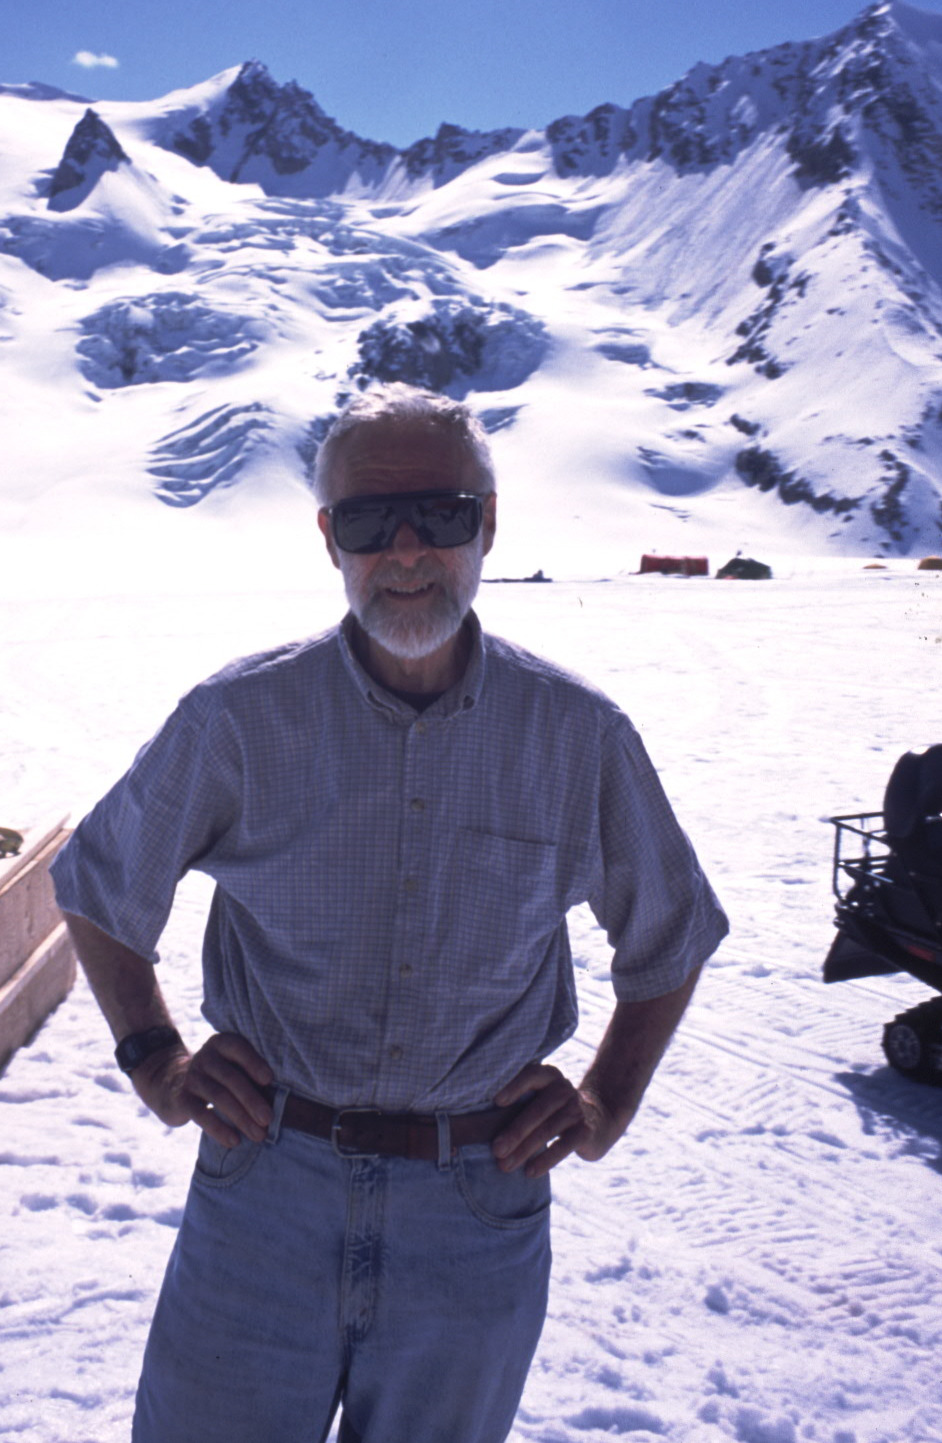
\includegraphics[width=0.8\textwidth]{figs/Will-by-Truffer.jpg}
%\url{https://news.uaf.edu/goodbye-to-a-raffish-glacier-scientist/}

\hfill \tiny \emph{photo by Martin Truffer} \phantom{dklfj asdlfj dslfaj}
\end{column}
\begin{column}{0.5\textwidth}
\begin{itemize}
\item W is a glaciologist
\invisible<1>{\item he is happy because he is standing on a glacier}
\invisible<1-2>{\item he can say two \emph{precise} things about his patch of the world}
\invisible<1-3>{\item one inequality and one equality}
\invisible<1-4>{\item<5>[$>$] the glacier thickness is positive
    $$H>0$$}

\vspace{-5mm}
\invisible<1-4>{\item<5>[$=$] the mass of ice is conserved
    $$\frac{\partial H}{\partial t} + \Div \left(\bU H\right) - a = 0$$}
\end{itemize}
\end{column}
\end{columns}
\end{frame}


\begin{frame}{A}

\begin{columns}
\begin{column}{0.5\textwidth}
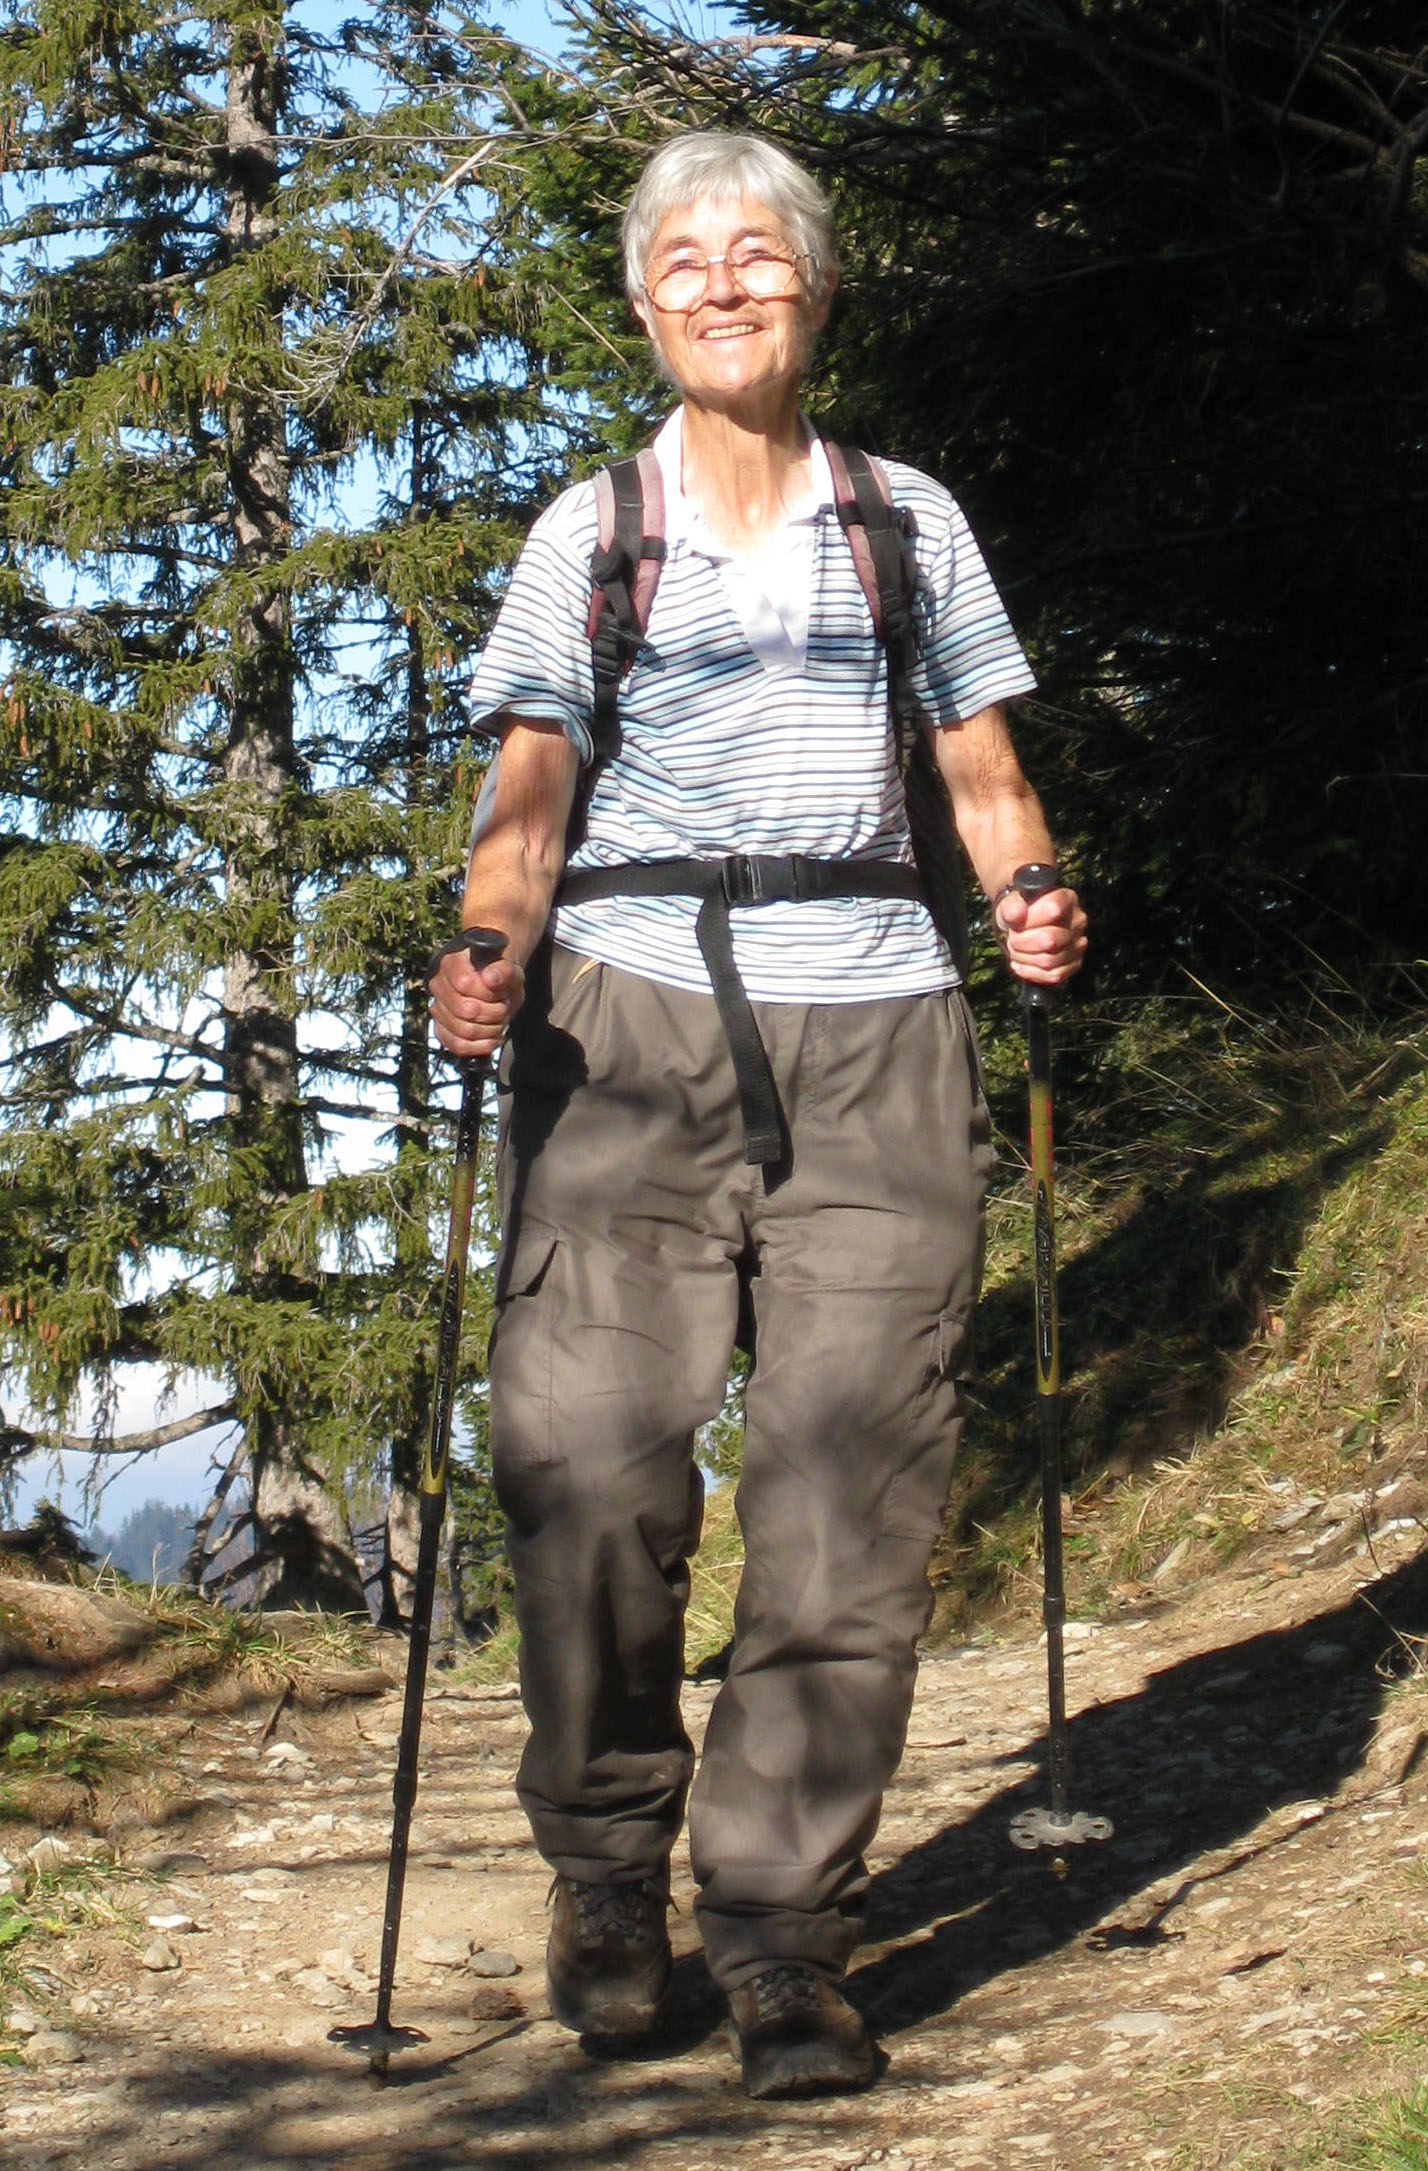
\includegraphics[width=0.8\textwidth]{figs/Iken_front_crop.jpg}
%\url{https://www.igsoc.org/awards/seligman/ikenseligman.html}
\end{column}
\begin{column}{0.5\textwidth}
\begin{itemize}
\item A is a glaciologist
\invisible<1>{\item she is not on a glacier, but happy to be hiking in the mountains}
\invisible<1-2>{\item she can say two \emph{precise} things about her patch of the world}
\invisible<1-3>{\item one equality and one inequality}
\invisible<1-4>{\item<5>[$=$] the glacier thickness is zero
    $$H=0$$}

\vspace{-5mm}
\invisible<1-4>{\item<5>[$>$] the annual surface mass balance is negative
    $$-a > 0$$}
\end{itemize}
\end{column}
\end{columns}
\end{frame}


\begin{frame}{two views in different patches}

\begin{columns}
\begin{column}{0.25\textwidth}
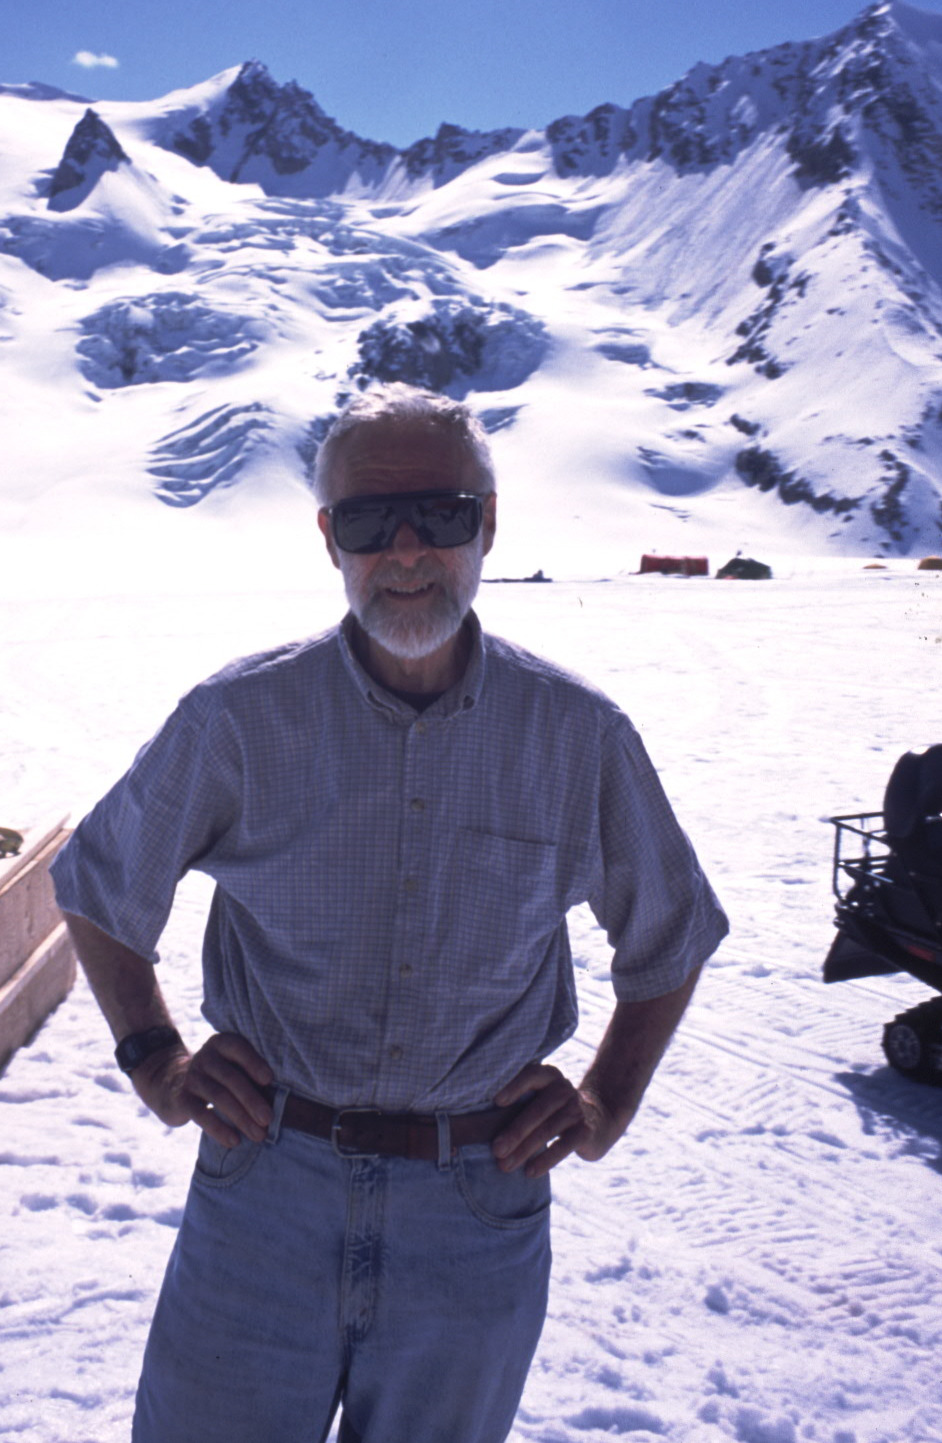
\includegraphics[width=0.7\textwidth]{figs/Will-by-Truffer.jpg}

\vspace{5mm}
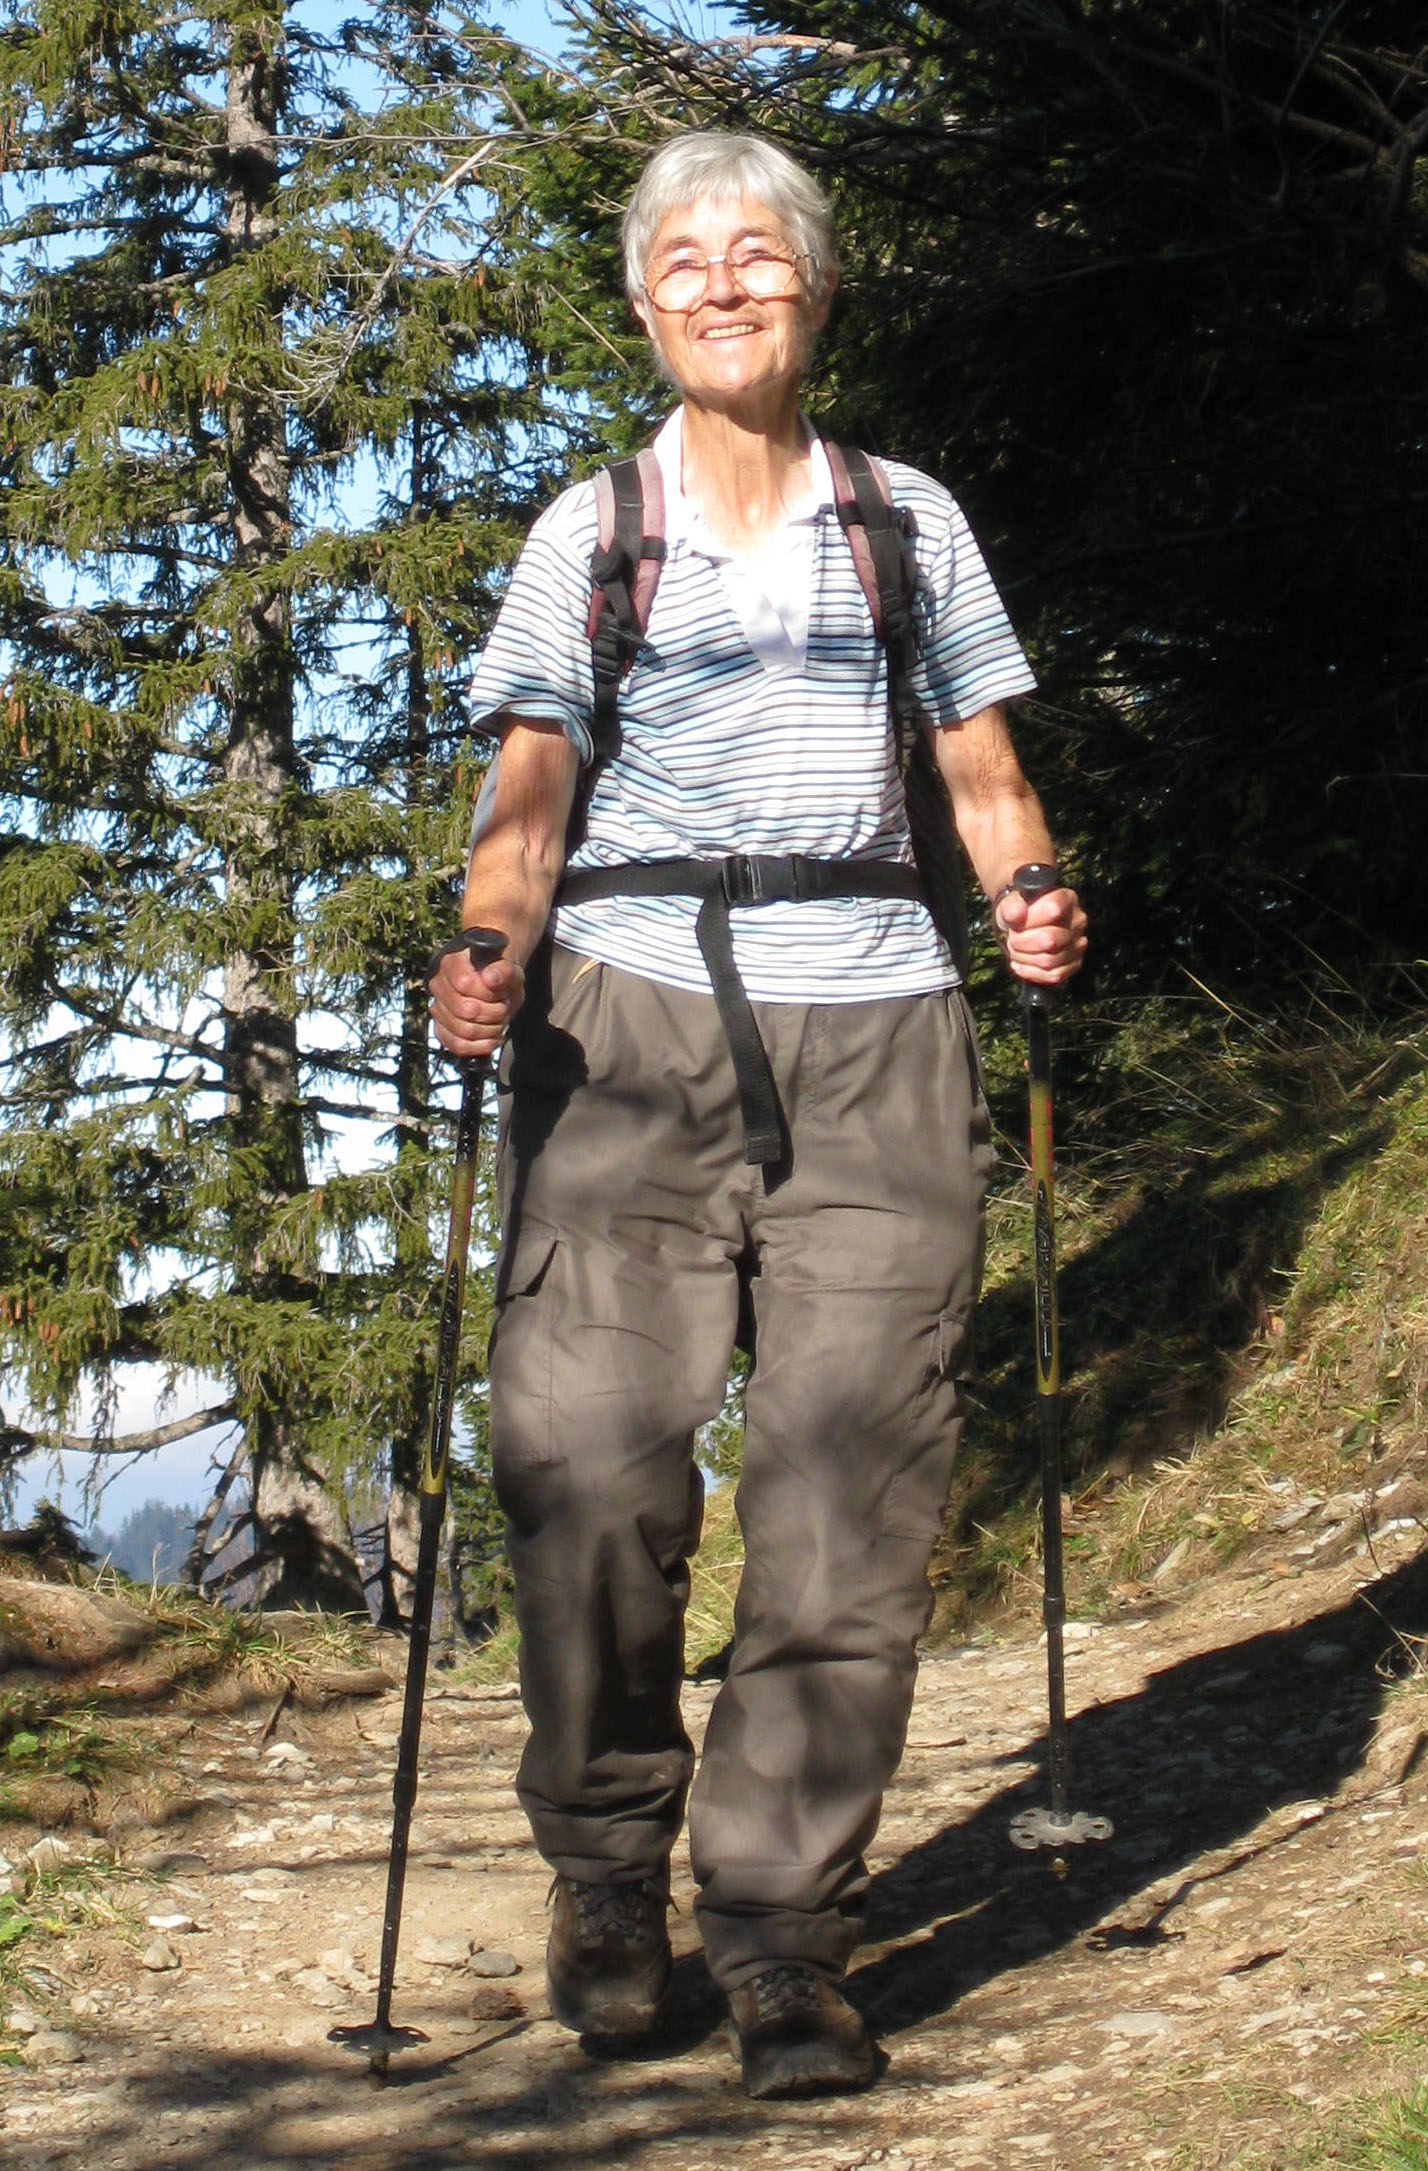
\includegraphics[width=0.7\textwidth]{figs/Iken_front_crop.jpg}

\bigskip

\bigskip
\end{column}
\begin{column}{0.75\textwidth}
\begin{itemize}
\item \emph{W says:} where I am
    \begin{itemize}
    \item[] the glacier thickness is positive
        $$H>0$$
    \item[] and mass of ice is conserved
        $$\frac{\partial H}{\partial t} + \Div \left(\bU H\right) - a = 0$$
    \end{itemize}
\item \emph{A says:} where I am
    \begin{itemize}
    \item[] the glacier thickness is zero
        $$H=0$$
    \item[] and the annual surface mass balance is negative
        $$-a > 0$$
    \end{itemize}

\medskip
\item<2> \emph{a skeptic says:} so what?  the world looks different in different places!
\end{itemize}
\end{column}
\end{columns}
\end{frame}


\begin{frame}{but first \dots define your terms}
\begin{itemize}
\item $\bx = (x,y)$ is map-plane location
\item $t$ is time

\medskip
\item $H(t,\bx)$ is glacier thickness
\item $b(\bx)$ is bed elevation (not changing)
\item $s(t,\bx)$ is glacier surface elevation
\item $a(t,\bx)$ is annual surface (climatic) mass balance
    \begin{itemize}
    \item[$\circ$] a.k.a.~the accumulation-ablation function
    \end{itemize}
\item $\bU = \bU(t,\bx)$ is vertically-averaged horizontal ice velocity
\item $\bu = \bu(t,x,y,z)$ is ice velocity in 3D
\end{itemize}

\vspace{20mm}

\footnotesize
\alert{the symbols are dumb, questions about them are not!}
\end{frame}


\begin{frame}{both views at once}
\begin{itemize}
\item both W's view and A's view arise from one set of equations:
\begin{align*}
H &\ge 0 \\
\frac{\partial H}{\partial t} + \Div \left(\bU H\right) - a &\ge 0 \\
H \left(\frac{\partial H}{\partial t} + \Div \left(\bU H\right) - a\right) &= 0
\end{align*}

\begin{itemize}
\item[$\circ$] \emph{consider}: W is standing on a glacier
\item[$\circ$] \emph{consider}: A is walking on a dirt trail
\end{itemize}

\invisible<1>{
\bigskip
\item<2> ``equations'' will mean ``set of equations and inequalities''
\item<2> the third equation is \alert{complementarity}
\item<2> the whole thing is a \alert{(nonlinear) complementarity problem}, an \alert{NCP}
}
\end{itemize}
\end{frame}


\section{complementarity for glaciers}

\begin{frame}{what is true at a glacier margin?}

\begin{center}
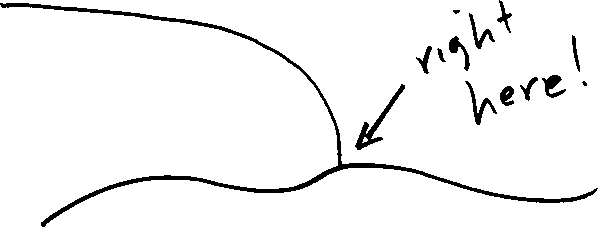
\includegraphics[width=0.4\textwidth]{figs/margin.png}
\end{center}

\begin{itemize}
\item one switches from W's view to A's view at a glacier margin
\only<1>{
\item an extra equality holds at a margin:
   $$H=0 \qquad \text{\emph{and}} \qquad \frac{\partial H}{\partial t} + \Div \left(\bU H\right) - a = 0$$
}
\only<2>{
\item \alert{an extra equality holds at a margin?}
   $$H=0 \qquad \text{\emph{and}} \qquad \frac{\partial H}{\partial t} + \Div \left(\bU H\right) - a \alert{\stackrel{?}{=}} 0$$
}
\end{itemize}
\end{frame}


\begin{frame}{useful to think about \emph{open sets}}

\begin{center}
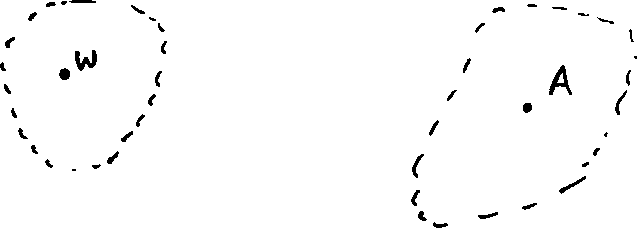
\includegraphics[width=0.4\textwidth]{figs/opensets.png}
\end{center}

\begin{itemize}
\item ``W is on a glacier'' means a neighborhood of glacier is around W
\item ``A is on a trail'' means a neighborhood of dirt is around A
\item ``neighborhood'' $=$ open set in the map-plane

\medskip
\item \emph{idea}:  a complementarity problem using derivatives, or any strong-form differential equation, only makes sense in open sets around locations

\medskip
\item but a glacier margin has no neighborhood of differentiability of $H$ or $\bU$,
\item \dots so let's not assume the NCP equations hold \emph{at} the margin
\end{itemize}
\end{frame}


\begin{frame}{velocity or flux?}
\begin{itemize}
\item \dots and you might be worried about the zen question:

\begin{center}
\emph{what is the velocity $\bU$ of a glacier that isn't there?}
\end{center}

\vspace{5mm}
\item<2> let $\bq$ be the map-plane \emph{mass flux}; it \emph{is} defined everywhere

\medskip
\item<2> \alert{$\bq = \bU H$ \emph{on the glacier}, but $H=0$ and $\bq=\bzero$ outside the glacier}

\medskip
\item<2> mass conservation equation says \quad $\frac{\partial H}{\partial t} + \Div \bq = a$ \quad \emph{on the glacier}

\medskip
\item<2> dynamics determines flow from geometry, so: \quad $\bq=\bq(H)$
    \begin{itemize}
    \item[$\circ$] we can agree?: \quad $\bq(0)=\bzero$
    \end{itemize}
\end{itemize}
\end{frame}


\begin{frame}{what is \emph{actually} true at a glacier margin?}

\begin{center}
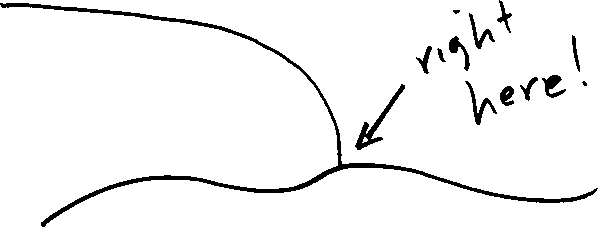
\includegraphics[width=0.4\textwidth]{figs/margin.png}
\end{center}

\bigskip
\begin{itemize}
\item \alert{both $H(t,\bx)$ and $\bq(t,\bx)$ are continuous in the map plane}
    \begin{itemize}
    \item[$\circ$] \dots in any fluids view of glaciers where thickness is well-defined
    \end{itemize}

\medskip
\item so $H=0$ \emph{and} $\bq=\bzero$ at a glacier margin
    \begin{itemize}
    \item[$\circ$] true whether the margin is advancing, stationary, or retreating
    \end{itemize}

\medskip
\item the quantity \quad $\frac{\partial H}{\partial t} + \Div \bq - a$ \quad jumps discontinuously
\end{itemize}
\end{frame}


\begin{frame}{applies everywhere, including where the glacier is}
\begin{itemize}
\item NCP = nonlinear complementarity problem
\item the glacier NCP applies \emph{everywhere on Earth}:
\begin{align*}
H &\ge 0 \\
\frac{\partial H}{\partial t} + \Div \bq - a &\ge 0 \\
H \left(\frac{\partial H}{\partial t} + \Div \bq - a\right) &= 0
\end{align*}
    \begin{itemize}
    \item[$\circ$] at the South Pole 1000 years ago
    \item[$\circ$] 1000 years from now in the middle of Death Valley
    \item[$\circ$] outside my door right now

    \medskip
    \item<2>[$\circ$] \emph{except} right at glacier margins
    \end{itemize}
\end{itemize}
\end{frame}


\begin{frame}{where be glaciers?}

\begin{columns}
\begin{column}{0.65\textwidth}
\begin{itemize}
\item ``where is there a glacier?'' is a first-class problem in glaciology
    \begin{itemize}
    \item[$\circ$] \emph{example}: determine ice sheet extent in hypothesized previous climate
    \end{itemize}
\item we want our theory and models to apply everywhere, so that we may answer this first-class problem \emph{within} a model
\item an NCP is such a model:
\begin{align*}
H &\ge 0 \\
\frac{\partial H}{\partial t} + \Div \bq - a &\ge 0 \\
H \left(\frac{\partial H}{\partial t} + \Div \bq - a\right) &= 0
\end{align*}
    \begin{itemize}
    \item[$\circ$] it remains to compute $\bq$ from geometry \dots via conservation of momentum
    \end{itemize}
\end{itemize}
\end{column}
\begin{column}{0.35\textwidth}
\hfill 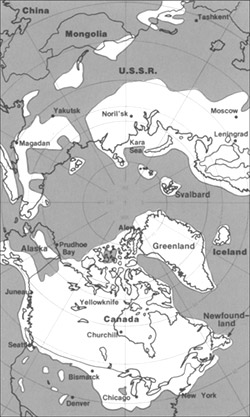
\includegraphics[width=0.9\textwidth]{figs/Pleistocene_north_ice_map.jpg}

\tiny

\hfill J.~Schlee

\hfill \mbox{\url{pubs.usgs.gov/gip/continents/}}
\end{column}
\end{columns}
\end{frame}


\begin{frame}{my main point}
\begin{itemize}
\item if you say ``my glacier model conserves mass'' then think
\begin{align*}
H &\ge 0 \\
\frac{\partial H}{\partial t} + \Div \bq - a &\ge 0 \\
H \left(\frac{\partial H}{\partial t} + \Div \bq - a\right) &= 0
\end{align*}
\emph{everywhere}, and not just
    $$\frac{\partial H}{\partial t} + \Div \bq = a$$
on the glacier

\medskip
\item<2> note $H$, $\bq$, $a$ can be defined everywhere
\end{itemize}
\end{frame}


\begin{frame}{mass conservation or surface kinematical equation?}
\begin{itemize}
\item \emph{recall}: $H$ is thickness, $s$ surface elevation, and $b$ bed elevation
    \begin{itemize}
    \item[$\circ$] $H=s-b$
    \item[$\circ$] $H_t=s_t$ because we have assumed $b_t=0$
    \end{itemize}
\item the mass conservation and surface kinematical equations are equivalent if the ice is incompressible
    $$\frac{\partial H}{\partial t} + \Div \bq - a = 0 \qquad \iff \qquad \frac{\partial s}{\partial t} - \bu \cdot \bn_s - a = 0$$
    \begin{itemize}
    \item[$\circ$] where $\bn_s = \left<-\frac{\partial s}{\partial x},-\frac{\partial s}{\partial y},1\right>$ is normal to the surface
    \end{itemize}

\bigskip
\scriptsize
\item[] \emph{justification in frozen and nonsliding case, using Leibniz rule and incompressibility:}
\begin{align*}
\Divbx \bq &= \Divbx \left(\int_b^s \left<u,v\right>\,dz\right) = \left<u,v\right>\big|_s \cdot \grad_{\bx} s - \left<u,v\right>\big|_b \cdot \grad_{\bx} b + \int_b^s \Divbx \left<u,v\right>\,dz \\
           &= \left<u,v\right>\big|_s \cdot \grad_{\bx} s - \int_b^s w_z\,dz = \left<u,v\right>\big|_s \cdot \grad_{\bx} s - w\big|_s = - \bu \cdot \bn_s
\end{align*}

\medskip
\normalsize
\item in sliding and/or melting base cases we use the (nontrivial) basal kinematical equation to get the \textbf{same} SKE, but the mass conservation equation is modified
\end{itemize}
\end{frame}


\begin{frame}{NCP using surface kinematical equation}

\begin{itemize}
\item the surface kinematical equation does not care about incompressibility or the basal motion
\item restated NCP:
\begin{align*}
s-b &\ge 0 \\
\frac{\partial s}{\partial t} - \bu \cdot \bn_s - a &\ge 0 \\
(s-b) \left(\frac{\partial s}{\partial t} - \bu \cdot \bn_s - a\right) &= 0
\end{align*}

\medskip
\item a bit better, but not really more fundamental
    \begin{itemize}
    \item[$\circ$] NCP form assumes $H$ and $s$ are well-defined, thus no overhangs, and this \emph{is} a fundamental restriction on glacier geometry
    \end{itemize}
\end{itemize}
\end{frame}


\section{complementarity from optimization}

\newcommand{\blambda}{\bm{\lambda}}

\begin{frame}{inequality-constrained optimization}
\begin{itemize}
\item I did not invent ``complementarity''
\item optimization problem:
    $$\min_{\bv\in\RR^n} \phi(\bv) \qquad \text{subject to} \qquad \bv \ge 0 \phantom{sd ad adsaf jsdlkja asdf kj asdf asdfa ad sdfa sad}$$

\vspace{-20mm}
\hfill 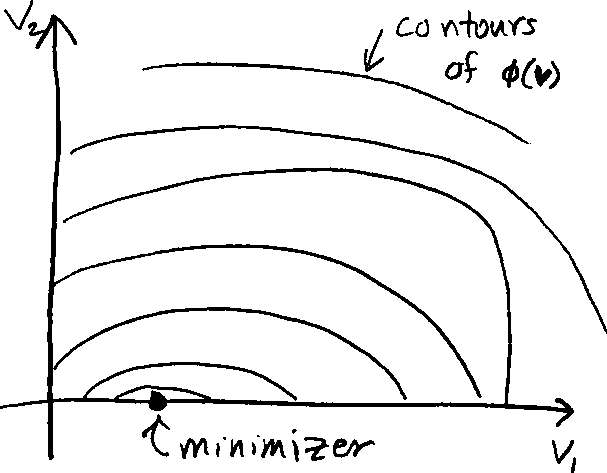
\includegraphics[width=0.35\textwidth]{figs/optimization.png}

\vspace{-8mm}
\item Lagrange multipliers:

\smallskip
\qquad $\Phi(\bv,\blambda) = \phi(\bv) - \blambda \cdot \bv$
\item then:
    $$\bv \ge 0, \qquad \blambda \ge 0, \qquad \grad \phi(\bv) - \blambda = 0, \qquad \bv\, \blambda = 0$$

    \begin{itemize}
    \item[$\circ$] these are KKT conditions; the last is \alert{complementary slackness}
    \end{itemize}
\item eliminate $\blambda$ and define $\bF(\bv) = \grad \phi(\bv)$ to state as NCP:
\begin{align*}
\bv &\ge 0 \\
\bF(\bv) &\ge 0 \\
\bv\, \bF(\bv) &= 0
\end{align*}
\end{itemize}
\end{frame}


\begin{frame}{example and analogy: obstacle problem}

\begin{center}
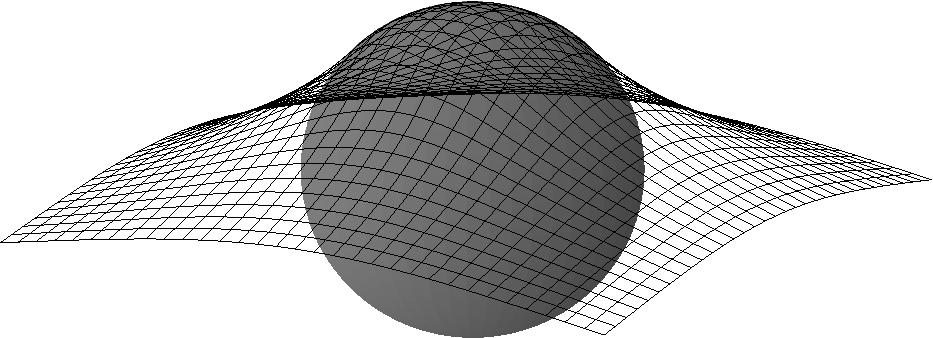
\includegraphics[width=0.6\textwidth]{figs/obstacle65.pdf}
\end{center}

\begin{itemize}
\item the well-known \emph{obstacle problem} is an $\infty$-dimensional NCP
    \begin{itemize}
    \item[$\circ$] just like the glacier problem
    \item[$\circ$] but it is also constrained optimization
    \end{itemize}
\item membrane position $u=u(\bx)$ solves:
    $$\min_{v} \phi(v) \qquad \text{subject to} \qquad v \ge \psi$$
where
    $$\phi(v) = \int_\Omega \frac{1}{2} |\grad v|^2 - f\, v\,d\bx$$

    \begin{itemize}
    \item[$\circ$] in the figure, $\Omega$ is a square, $\psi$ is the grey upper hemisphere, $f=0$, and the solution $u$ is shown as a mesh
    \item[$\circ$] $u$ and $v$ live in a space of functions on $\Omega$
        \begin{itemize}
        \item[$\vartriangleright$] such as $H_g^1(\Omega)$ where $g$ gives boundary values
        \end{itemize}                
    \end{itemize}
\end{itemize}
\end{frame}


\begin{frame}{no one wants a variational inequality?}

\hfill 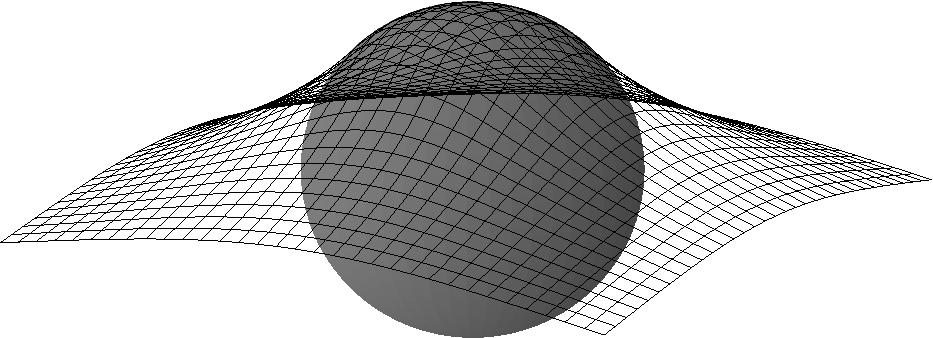
\includegraphics[width=0.35\textwidth]{figs/obstacle65.pdf}

\vspace{-15mm}
\begin{itemize}
\item equivalent obstacle problem formulations:
\begin{align*}
    \text{CO}& &&u = \min_{v} \phi(v) \quad \text{s.t. } v \ge \psi \\
    & \\
    \text{VI}& &&\int_\Omega \grad u \cdot \grad(v-u)\,d\bx \ge \int_\Omega f(v-u)\,d\bx \quad \text{for all } v \ge \psi \\
    & \\
   \text{NCP}& &&\begin{aligned} u - \psi &\ge 0 \\
                                 -\grad^2 u - f &\ge 0 \\
                                 (u - \psi) ( -\grad^2 u - f) &= 0 \end{aligned}
\end{align*}
\item VI $=$ \emph{variational inequality}
\item I've concluded nobody really thinks VI style
\item NCPs are easier to understand, both for scientists and mathematicians
\item of course, CO $=$ \emph{constrained optimization} is pretty intuitive \dots
\end{itemize}
\end{frame}


\begin{frame}{the glacier problem is not optimization}

\begin{itemize}
\item unfortunately, glaciers do not optimize any energy functional
    \begin{itemize}
    \item[$\circ$] no such energy has been offered; for known theories the necessary symmetry is missing
    \end{itemize}

\medskip
\item obstacle problem:

\medskip
\hspace{20mm} CO $\leftrightarrow$ VI $\leftrightarrow$ NCP

\smallskip
\item glacier problem has no optimization form:

\smallskip
\hspace{20mm} \phantom{CO $\leftrightarrow$} VI $\leftrightarrow$ NCP

\medskip
\item so I'm stuck explaining using NCP
\item at least NCP is a ``strong form'' (pointwise statements) while CO and VI are ``weak forms'' (integrals)
\end{itemize}
\end{frame}


\begin{frame}{how about all the other glacier equations?}
\begin{itemize}
\item momentum/energy conservation equations only apply within the glacier
\item for this talk their ``purpose'' is to provide velocity in the NCP:
    $$(\text{geometry, boundary stress, thermal state}) \implies \bU,\bq,\bu$$
\item i.e.
\begin{align*}
s-b &\ge 0 \\
\frac{\partial s}{\partial t} - \bu_{\text{from solving the mass/momentum/energy coupled problem}} \cdot \bn_s - a &\ge 0 \\
(s-b) \left(\frac{\partial s}{\partial t} - \bu_{\text{from solving the mass/momentum/energy coupled problem}} \cdot \bn_s - a\right) &= 0
\end{align*}
\item my current project: make it work with Stokes dynamics
\end{itemize}
\end{frame}


\begin{frame}{steady state and implicit time steps}
\begin{itemize}
\item if a glacier is in steady state with a steady climate $a$ then
\begin{align*}
s-b &\ge 0 \\
- \bu \cdot \bn_s - a &\ge 0 \\
(s-b) \left(- \bu \cdot \bn_s - a\right) &= 0
\end{align*}
\item if we want to solve for $s$ after a backward Euler step of $\Delta t$ then
\begin{align*}
s-b &\ge 0 \\
s - s_{\text{old}} - \Delta t\left(\bu \cdot \bn_s + a\right) &\ge 0 \\
(s-b) \left(s - s_{\text{old}} - \Delta t\left(\bu \cdot \bn_s + a\right)\right) &= 0
\end{align*}
\item \emph{no problem stating NCPs for these situations}
    \begin{itemize}
    \item[$\circ$] plus well-posedness proofs in some particular cases
    \end{itemize}
\item but for explicit steps there are regularity issues
    \begin{itemize}
    \item[$\circ$] a separate discussion
    \end{itemize}
\end{itemize}
\end{frame}


\section{consequences/advantages for modelers (\emph{and real people})}

\begin{frame}{an NCP is a sanity check on your evolving glacier model}
\begin{itemize}
\item FIXME 
\end{itemize}
\end{frame}

\begin{frame}{the NCP is the source of margin shape}
\begin{itemize}
\item FIXME 
\end{itemize}
\end{frame}


\begin{frame}{an NCP is something you can run on a computer}
\begin{itemize}
\item FIXME works with NCP solver and Newton method as in SIAFVE: provide $a$ and $b$ on $\Omega$, give initial guess for $s$, and say ``go''
\item FIXME current project: make it Stokes
\item for implicit time steps
\end{itemize}
\end{frame}


\begin{frame}{a Newton step in an NCP}

\begin{columns}
\begin{column}{0.7\textwidth}
\begin{itemize}
\item FIXME think through what a Newton step looks like
\end{itemize}
\end{column}
\begin{column}{0.3\textwidth}
\hfill 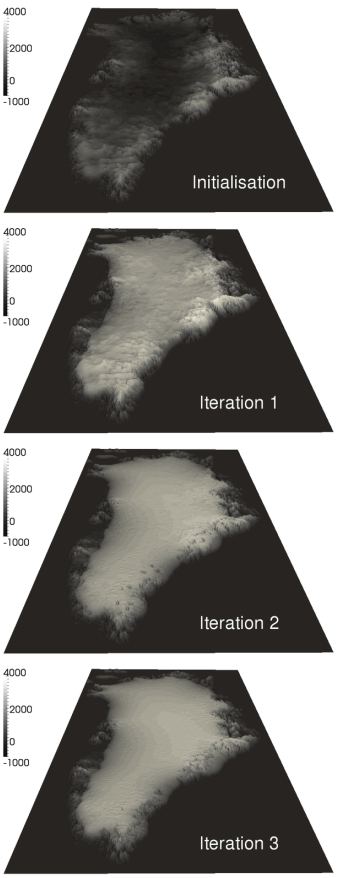
\includegraphics[width=0.8\textwidth]{figs/GISsequence.png} \hfill
\end{column}
\end{columns}
\end{frame}


\begin{frame}{discrete mass conservation will fail}
\begin{itemize}
\item when solving an NCP, discrete mass conservation will fail
\item FIXME at the free boundary is impossible; see layer paper
\item however, bounds on mass accounting errors
\end{itemize}
\end{frame}


\begin{frame}{A's view as logic}

\begin{columns}
\begin{column}{0.8\textwidth}
\begin{itemize}
\item even on a dirt trail, precise glaciology is possible:

\bigskip
\begin{quote}
If the glacier thickness is zero where you are then the annual surface mass balance cannot be positive.
\end{quote}
\end{itemize}
\end{column}
\begin{column}{0.2\textwidth}
\hfill 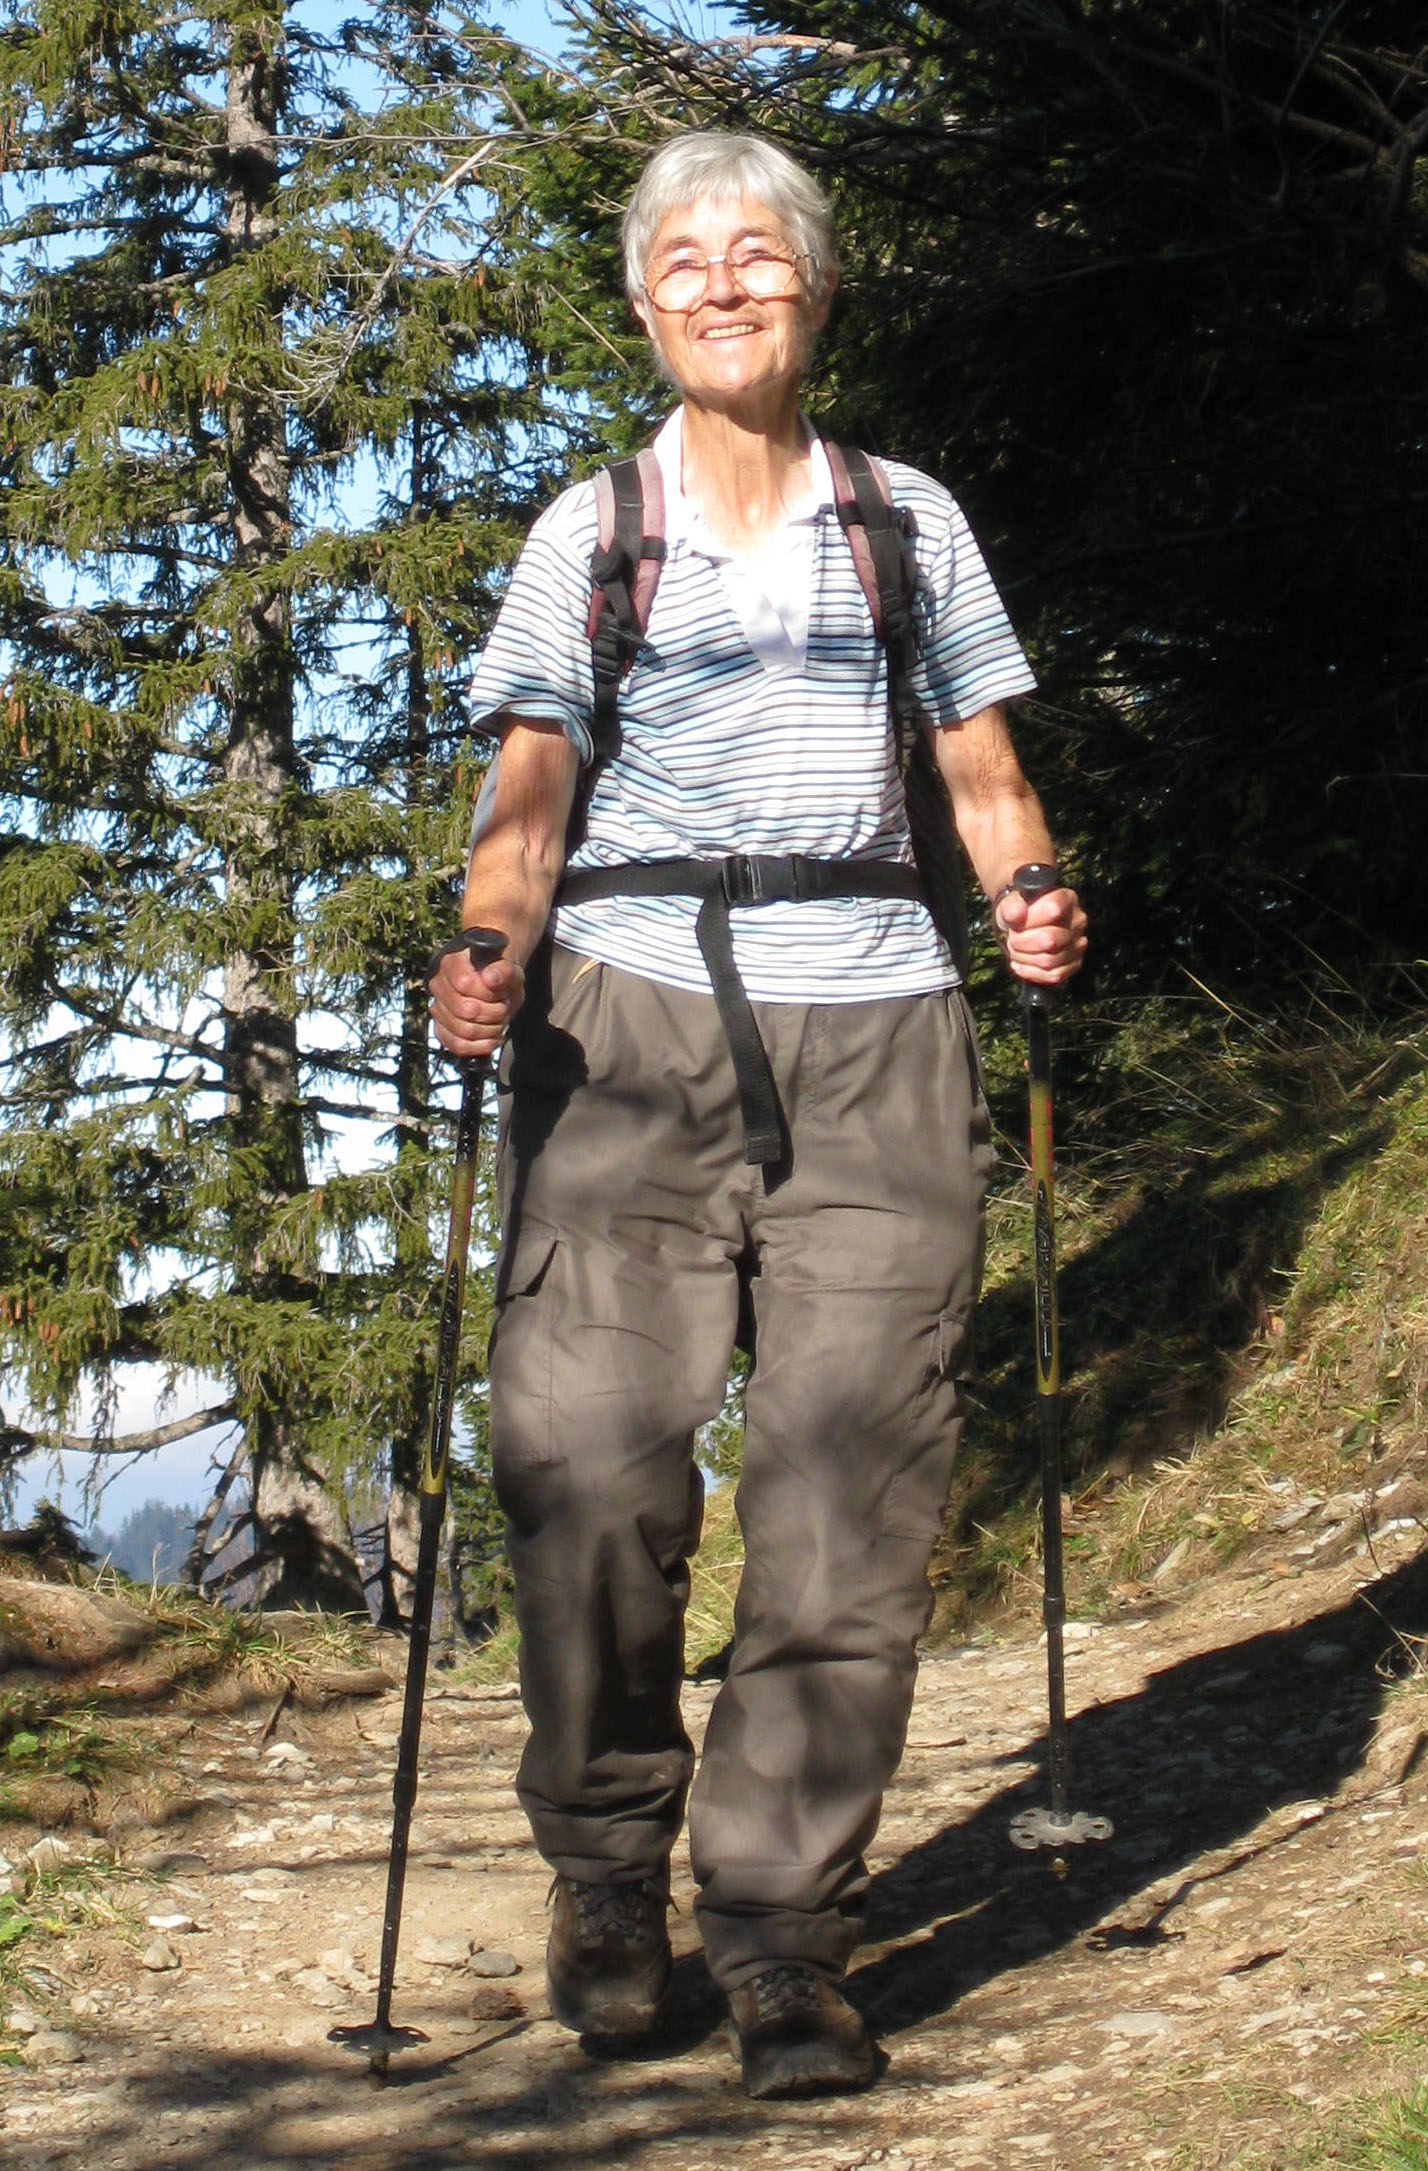
\includegraphics[width=0.7\textwidth]{figs/Iken_front_crop.jpg} \hfill
\end{column}
\end{columns}

\begin{itemize}
\item we already knew that?
\item the glossary\footnote{IACS Working Group, \emph{Glossary of glacier mass balance and related terms}, 2011} could redefine \emph{annual (climatic) surface mass balance} $a$ as any quantity which makes the NCP true
\begin{align*}
s-b &\ge 0 \\
\frac{\partial s}{\partial t} - \bu \cdot \bn_s - a &\ge 0 \\
(s-b) \left(\frac{\partial s}{\partial t} - \bu \cdot \bn_s - a\right) &= 0
\end{align*}

\vspace{-2mm}
    \begin{itemize}
    \item[$\circ$] this gives meaning to modeled values for $a$ outside the current glacier, not just prior measurements \emph{on} the glacier
    \end{itemize}
\end{itemize}
\end{frame}


\begin{frame}{surface mass balance should be modeled (almost) everywhere}
\begin{itemize}
\item to numerically compute the steady state of a glacier in a model, or for an implicit time step, it is essential that the modeled surface mass balance be available not just \emph{on} the glacier but everywhere
    \begin{itemize}
    \item[$\circ$] or at least ``nearby''
    \item[$\circ$] garbage in, garbage out
    \end{itemize}
\item in an energy balance model, for example, it requires a ``thought experiment'' for (e.g.) a dirt trail area:

\begin{quotation}
how fast would a piston of bare ice or snow need to rise in order

to stay at this level in this climate?
\end{quotation}
\end{itemize}

\begin{center}
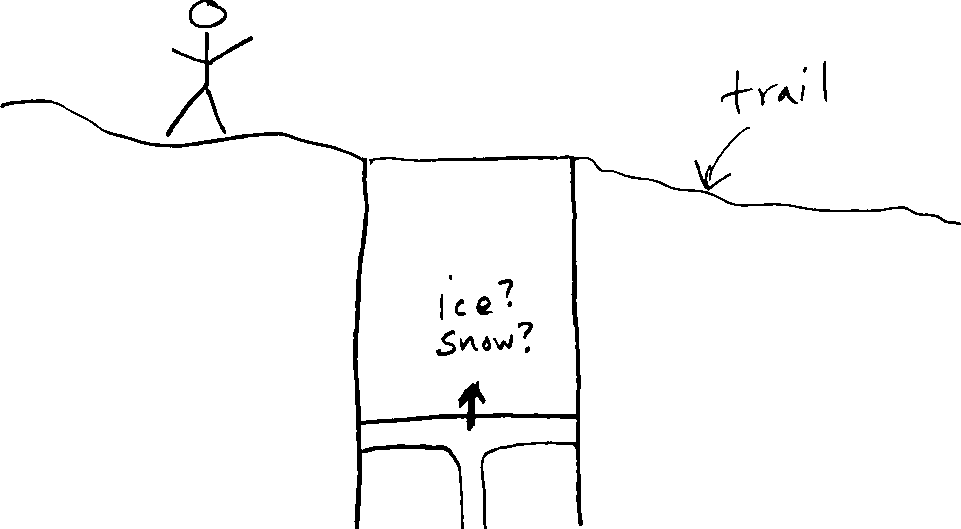
\includegraphics[width=0.5\textwidth]{figs/pistontrail.png}
\end{center}
\end{frame}


\begin{frame}{are there big ideas in glaciology?}
\begin{itemize}
\item I am not sure most glaciologists have an opinion on this
\item<2-4> I disagree

\bigskip
\item<3-4> some possible ``big ideas'':
    \begin{itemize}
    \item[$\circ$] volume-area scaling
    \item[$\circ$] hysteresis from elevation-dependent mass balance
    \item[$\circ$] the tidewater glacier cycle
    \item[$\circ$] why glaciers surge
    \end{itemize}
\item<3-4> none of these are obvious even to smart non-glacier scientists

\bigskip
\item<4> add ``complementarity gives glacier extent'' to list?
\end{itemize}
\end{frame}


\begin{frame}{remembering}

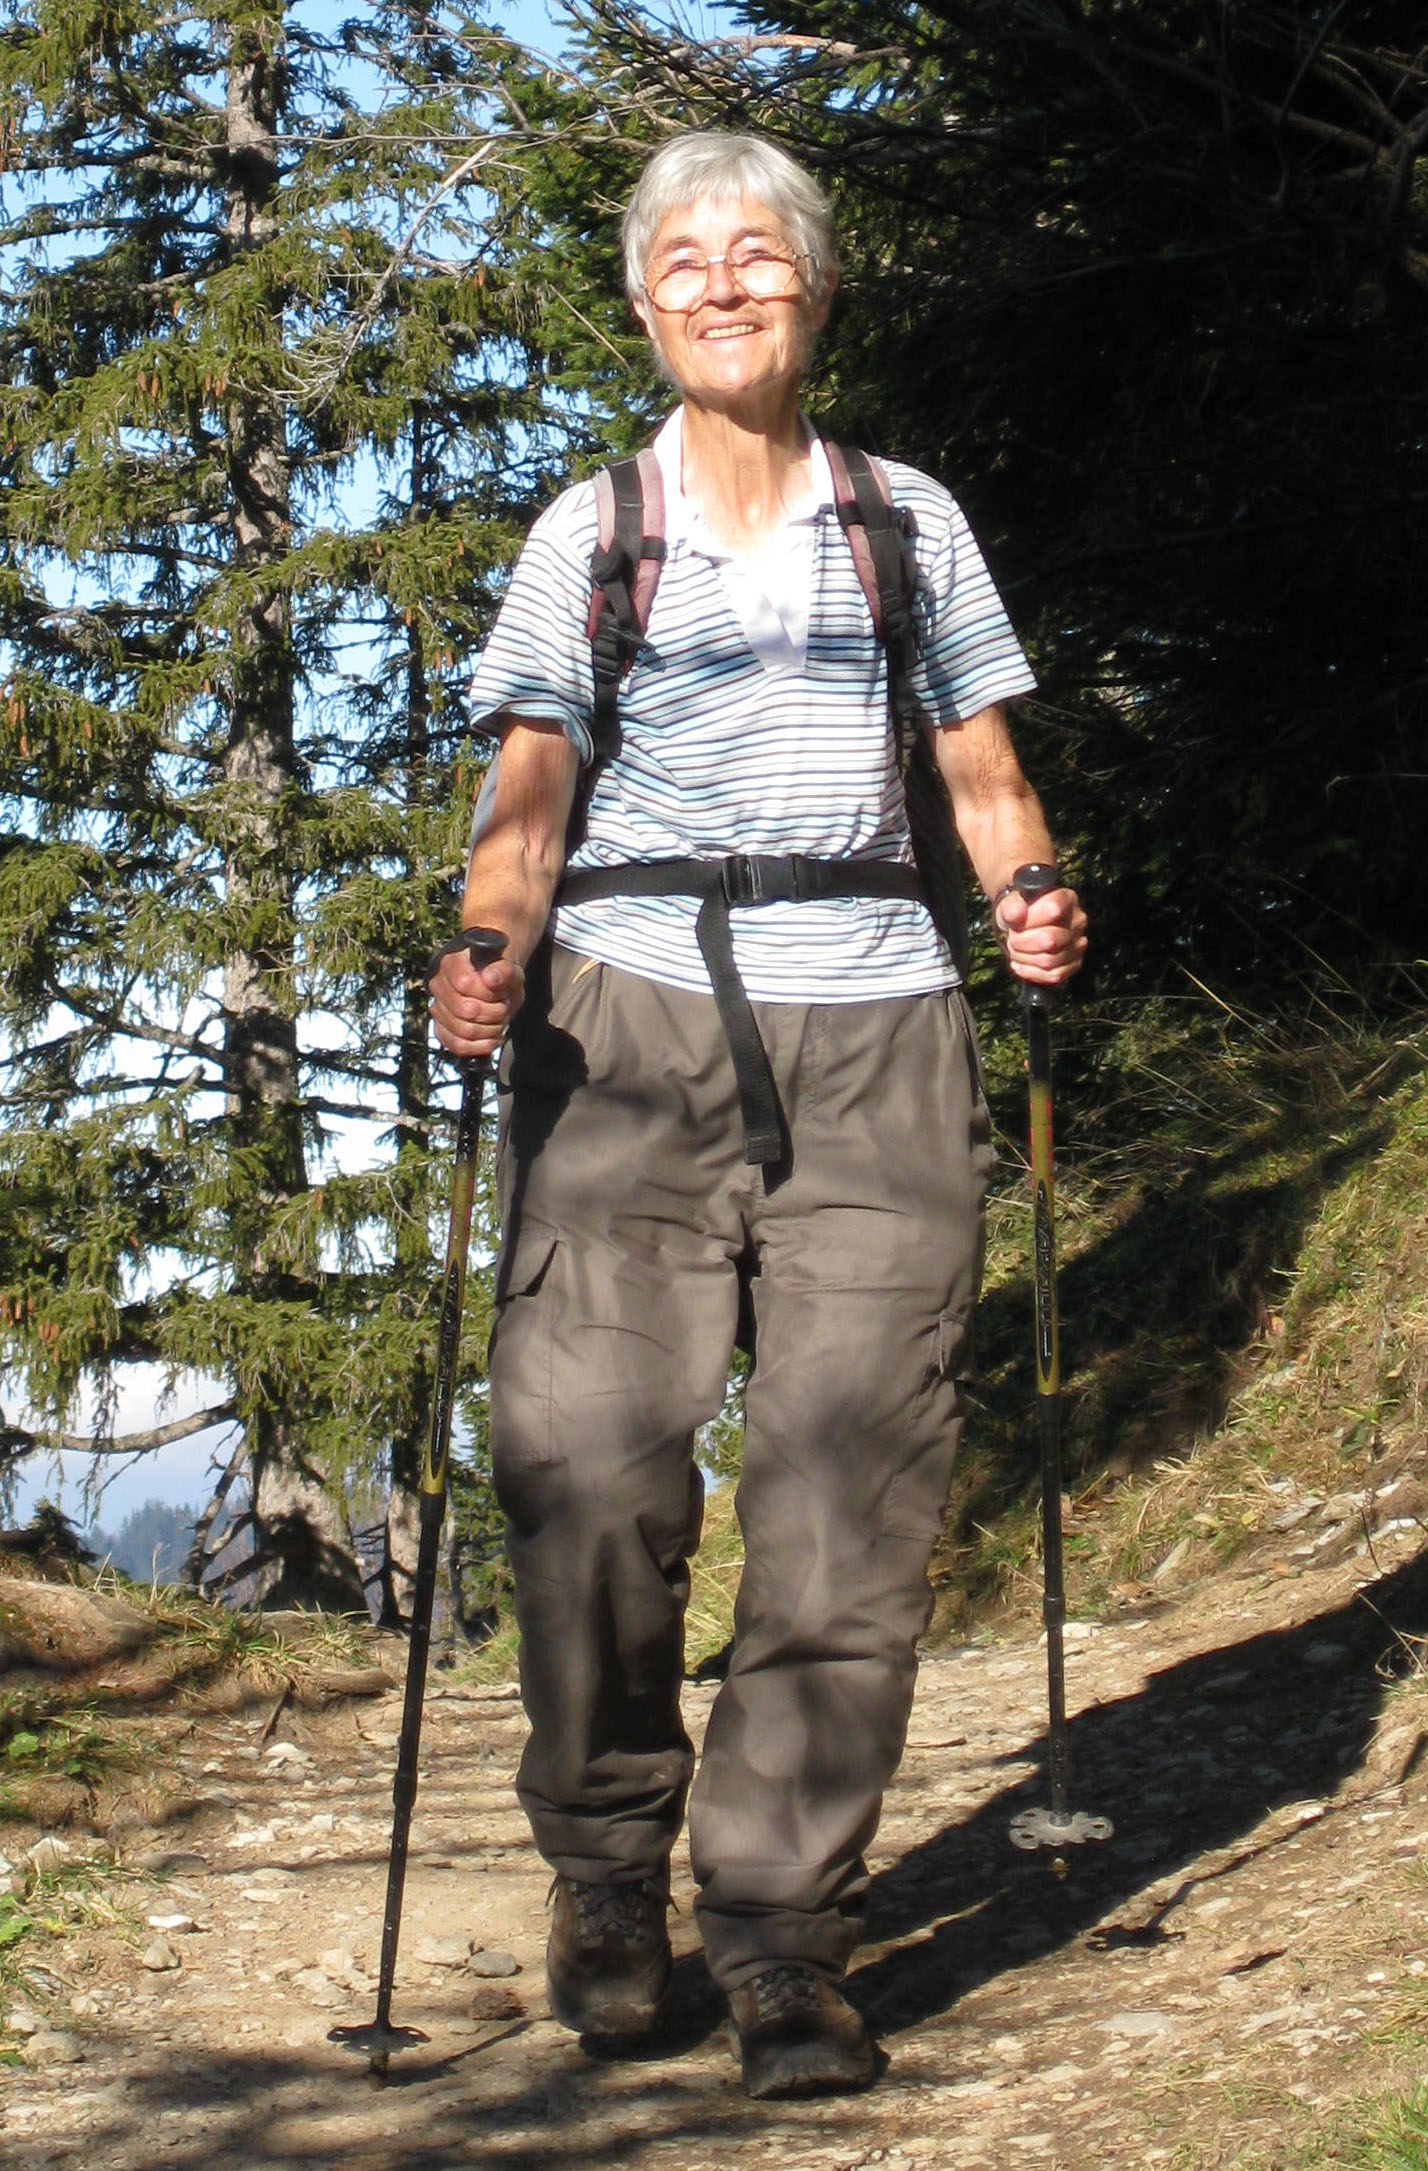
\includegraphics[width=0.4\textwidth]{figs/Iken_front_crop.jpg} \hfill 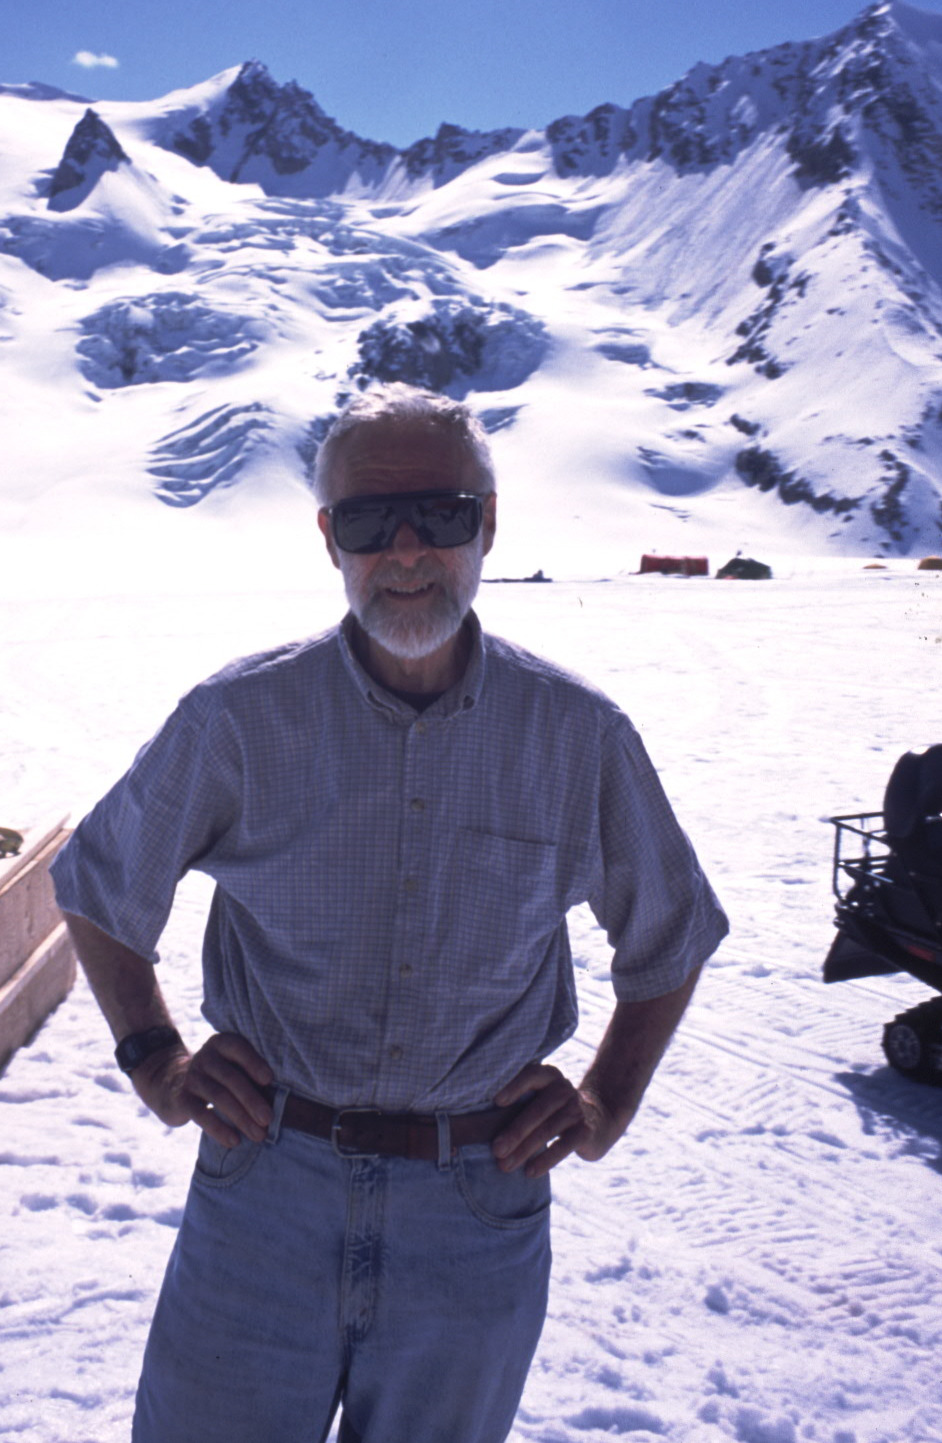
\includegraphics[width=0.4\textwidth]{figs/Will-by-Truffer.jpg}

Almut Iken (1933--2018) \hfill Will Harrison (1936--2020)
\end{frame}


\end{document}

